% ============================================================
% ARCHIVED SECTIONS (3-7) from document.tex
% Sections: Description des données, Exploration des données,
%           Prétraitement, Modélisation, Résultats et interprétation
% ============================================================

\section{Description des données}

Quatre sources de données ont été mises à disposition par le service RH de HumanForYou. L'ensemble des sources partagent la clé \texttt{EmployeeID} et entretiennent une relation 1:1, permettant une fusion par jointures successives (LEFT JOIN).

\subsection{Données générales (\texttt{general\_data.csv})}

Ce fichier constitue le socle du jeu de données avec \textbf{4\,410 employés} décrits par \textbf{24 variables}.

\begin{table}[htbp]
\centering
\caption{Variables principales du fichier \texttt{general\_data.csv}}
\small
\begin{tabularx}{\textwidth}{l l X}
\toprule
\textbf{Variable} & \textbf{Type} & \textbf{Description} \\
\midrule
Age & Numérique & Âge de l'employé \\
Attrition & Catégorielle & Variable cible (Yes/No) : départ en 2016 \\
BusinessTravel & Catégorielle & Fréquence des déplacements professionnels \\
Department & Catégorielle & Département (Sales, R\&D, HR) \\
DistanceFromHome & Numérique & Distance domicile--travail (km) \\
Education & Ordinale & Niveau d'éducation (1 à 5) \\
EducationField & Catégorielle & Domaine d'études \\
EmployeeCount & Constante & Toujours égal à 1 \\
EmployeeID & Identifiant & Clé primaire \\
Gender & Catégorielle & Genre (Male/Female) \\
JobLevel & Ordinale & Niveau hiérarchique (1 à 5) \\
JobRole & Catégorielle & Intitulé du poste \\
MaritalStatus & Catégorielle & Statut marital \\
MonthlyIncome & Numérique & Salaire mensuel (INR) \\
NumCompaniesWorked & Numérique & Nombre d'entreprises précédentes \\
Over18 & Constante & Toujours Y \\
PercentSalaryHike & Numérique & Pourcentage d'augmentation salariale \\
StandardHours & Constante & Toujours 8 \\
StockOptionLevel & Ordinale & Niveau de stock-options (0 à 3) \\
TotalWorkingYears & Numérique & Années d'expérience totale \\
TrainingTimesLastYear & Numérique & Formations suivies l'année précédente \\
YearsAtCompany & Numérique & Ancienneté dans l'entreprise \\
YearsSinceLastPromotion & Numérique & Années depuis la dernière promotion \\
YearsWithCurrManager & Numérique & Années avec le manager actuel \\
\bottomrule
\end{tabularx}
\end{table}

\textit{Note :} les variables \texttt{EmployeeCount}, \texttt{Over18} et \texttt{StandardHours} sont constantes et n'apportent aucune information discriminante ; elles seront supprimées lors du prétraitement.

\subsection{Enquête employé (\texttt{employee\_survey\_data.csv})}

Enquête soumise en juin 2015 (réponse non obligatoire). Trois questions notées sur une échelle de Likert de 1 à 4 :
\begin{itemize}
    \item \texttt{EnvironmentSatisfaction} : satisfaction vis-à-vis de l'environnement de travail ;
    \item \texttt{JobSatisfaction} : satisfaction vis-à-vis du travail ;
    \item \texttt{WorkLifeBalance} : équilibre vie professionnelle / vie personnelle.
\end{itemize}

\subsection{Évaluation manager (\texttt{manager\_survey\_data.csv})}

Dernière évaluation de chaque employé par son manager (février 2015) :
\begin{itemize}
    \item \texttt{JobInvolvement} : niveau d'implication au travail (1 à 4) ;
    \item \texttt{PerformanceRating} : évaluation de la performance annuelle (1 à 4).
\end{itemize}

\subsection{Horaires de badgeage (\texttt{in\_out\_time/})}

Deux fichiers (\texttt{in\_time.csv} et \texttt{out\_time.csv}) contenant les horodatages d'arrivée et de départ pour chaque jour ouvré de 2015 (261 jours). Ces données brutes ont été agrégées en \textbf{six indicateurs} par employé :

\begin{table}[htbp]
\centering
\caption{Variables dérivées des horaires de badgeage}
\small
\begin{tabularx}{\textwidth}{l X}
\toprule
\textbf{Variable} & \textbf{Description} \\
\midrule
\texttt{avg\_in\_hour} & Heure d'arrivée moyenne (format décimal) \\
\texttt{avg\_out\_hour} & Heure de départ moyenne \\
\texttt{avg\_work\_hours} & Durée de travail journalière moyenne \\
\texttt{std\_work\_hours} & Écart-type de la durée de travail (régularité) \\
\texttt{nb\_days\_present} & Nombre de jours de présence en 2015 \\
\texttt{nb\_days\_absent} & Nombre de jours d'absence en 2015 \\
\bottomrule
\end{tabularx}
\end{table}

\subsection{Jeu de données fusionné (\texttt{dataset\_final.csv})}

La fusion des quatre sources produit un jeu de données unique de \textbf{4\,410 lignes} et \textbf{35 colonnes}, réalisée par jointures LEFT JOIN successives sur \texttt{EmployeeID}. Le script \texttt{build\_dataset.py} automatise cette opération.

% ============================================================
\section{Exploration des données}

Cette section synthétise les résultats de l'analyse exploratoire (EDA) en se concentrant sur les constats qui orientent directement le prétraitement, la modélisation et les recommandations.

\subsection{Déséquilibre de la variable cible}

Sur les 4\,410 employés, \textbf{711 ont quitté l'entreprise} en 2016, soit un taux d'attrition de \textbf{16,1\,\%} (figure~\ref{fig:attrition_distribution}). Ce ratio 84/16 constitue un déséquilibre modéré qui devra être traité lors de la modélisation (rééchantillonnage, pondération des classes, ou choix de métriques adaptées comme le F1-score et l'AUC-ROC plutôt que l'accuracy).

\begin{figure}[htbp]
\centering
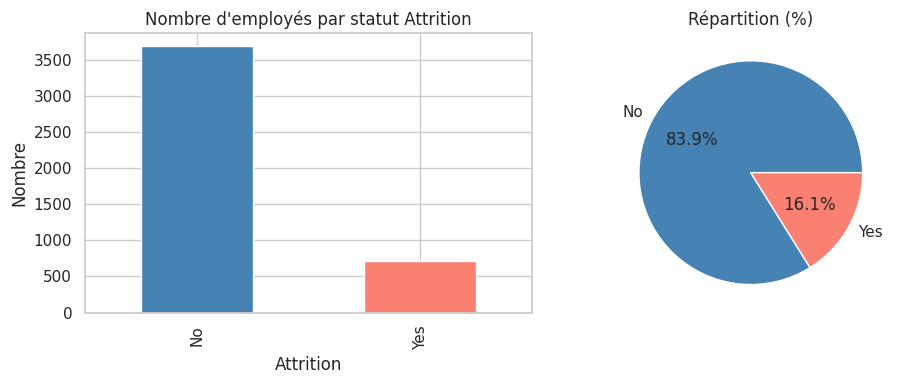
\includegraphics[width=0.85\textwidth]{figures/fig_attrition_distribution.png}
\caption{Distribution de la variable cible Attrition (effectifs et proportions)}
\label{fig:attrition_distribution}
\end{figure}

\subsection{Qualité des données}

Le jeu de données est de bonne qualité. Cinq variables présentent des valeurs manquantes, toutes à moins de 1\,\% : \texttt{WorkLifeBalance} (38), \texttt{EnvironmentSatisfaction} (25), \texttt{JobSatisfaction} (20), \texttt{NumCompaniesWorked} (19) et \texttt{TotalWorkingYears} (9). Une imputation simple (médiane ou mode) suffira. Trois variables sont constantes et seront supprimées : \texttt{EmployeeCount} (toujours 1), \texttt{Over18} (toujours Y) et \texttt{StandardHours} (toujours 8). De même, \texttt{PerformanceRating} ne prend que les valeurs 3 et 4 (aucune note inférieure à 3), ce qui en fait un signal très peu discriminant. Enfin, \texttt{avg\_in\_hour} présente un écart-type de seulement 0,02\,h (tous les employés arrivent à 10\,h) et pourra être écartée au profit de \texttt{avg\_work\_hours}.

\subsection{Facteurs d'attrition : variables catégorielles}

L'analyse du taux d'attrition par sous-groupe (figure~\ref{fig:attrition_by_category}) révèle trois populations à risque nettement au-dessus de la moyenne de 16,1\,\% :

\begin{itemize}
    \item Le département \textbf{Human Resources} : 30,2\,\%, soit presque le double de la moyenne ;
    \item Les employés \textbf{célibataires} : 25,5\,\%, contre 10,1\,\% pour les divorcés ;
    \item Les \textbf{voyageurs fréquents} : 24,9\,\%, soit trois fois plus que les sédentaires (8,0\,\%).
\end{itemize}

En revanche, l'écart entre hommes et femmes est faible (16,7\,\% vs 15,3\,\%), ce qui est rassurant du point de vue de l'équité du modèle.

\begin{figure}[htbp]
\centering
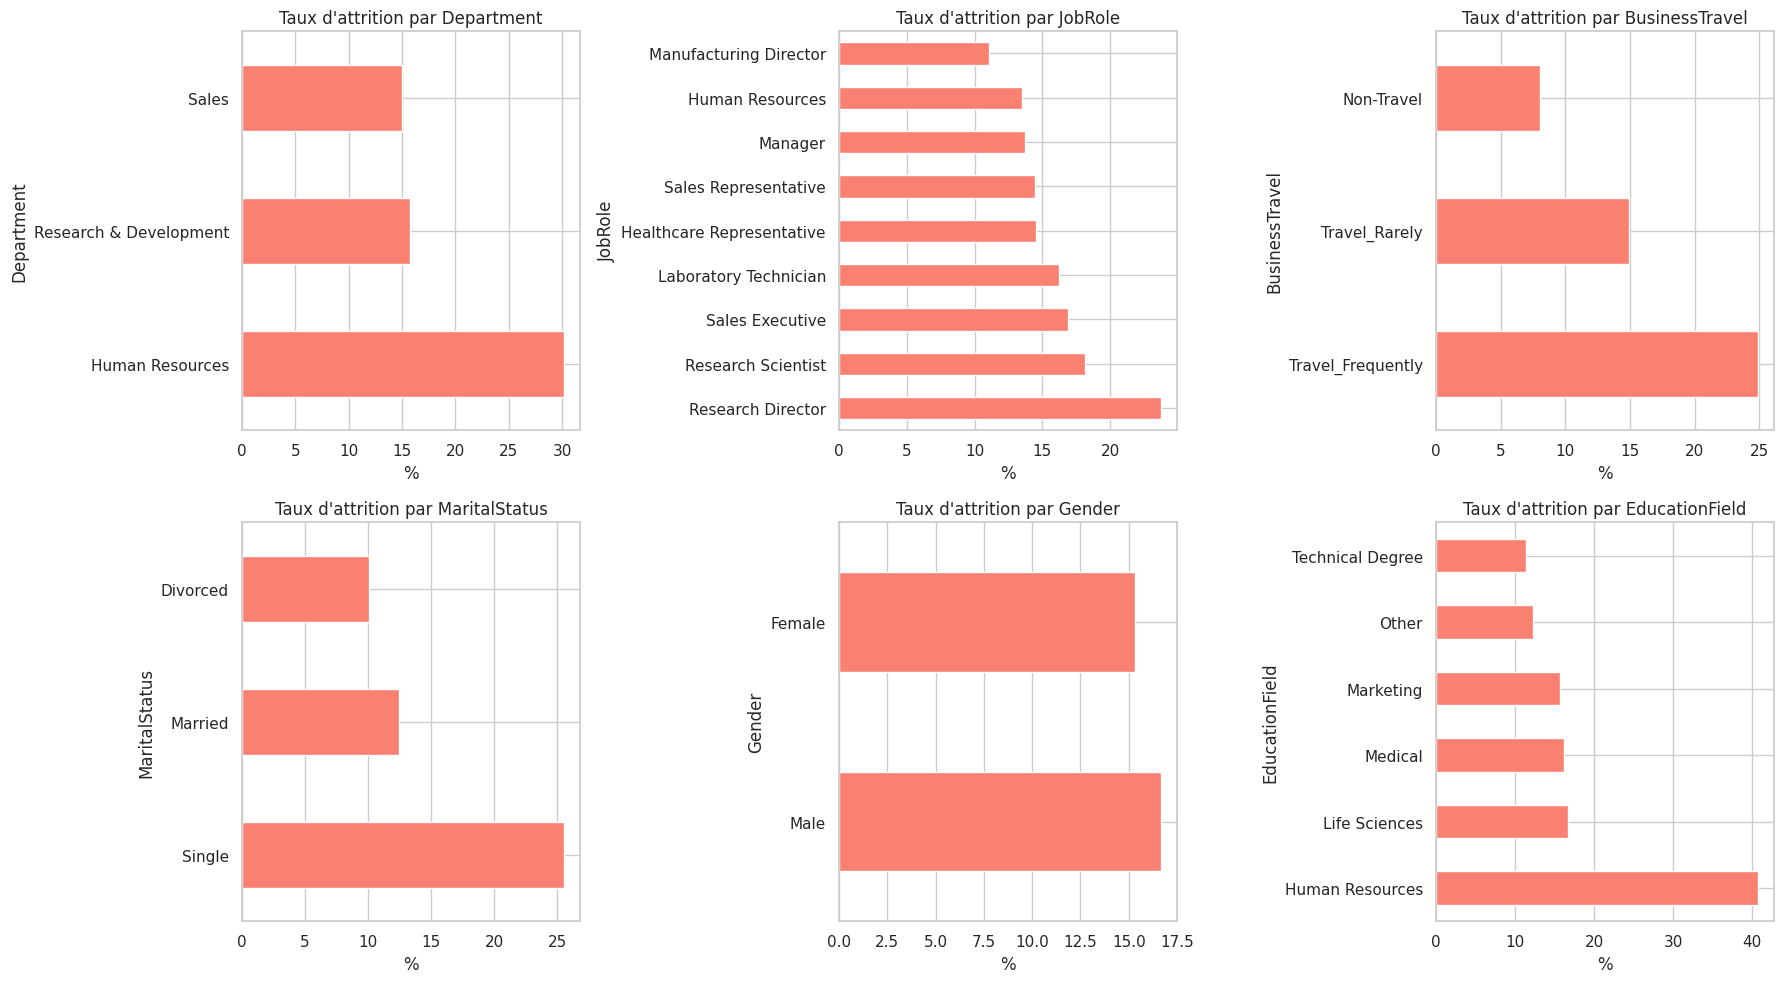
\includegraphics[width=\textwidth]{figures/fig_attrition_by_category.png}
\caption{Taux d'attrition par variable catégorielle --- les barres les plus longues identifient les populations à risque}
\label{fig:attrition_by_category}
\end{figure}

\subsection{Facteurs d'attrition : variables numériques}

La comparaison des moyennes entre employés partis et restés (tableau~\ref{tab:comparaison_moyennes}) met en évidence les variables les plus discriminantes. Les employés ayant quitté l'entreprise sont en moyenne \textbf{plus jeunes} ($-$4 ans), avec \textbf{moins d'ancienneté} ($-$2,2 ans), \textbf{moins d'expérience} ($-$3,6 ans) et une relation plus courte avec leur manager ($-$1,5 ans). Le résultat le plus marquant concerne la \textbf{durée de travail} : les partants travaillaient 8,32\,h/jour contre 7,58\,h pour les restants, soit \textbf{45 minutes de plus par jour} (figure~\ref{fig:numeric_distributions}).

\begin{table}[htbp]
\centering
\caption{Moyennes des variables numériques selon le statut d'attrition}
\label{tab:comparaison_moyennes}
\small
\begin{tabular}{l r r r}
\toprule
\textbf{Variable} & \textbf{Partis (Yes)} & \textbf{Restés (No)} & \textbf{Écart} \\
\midrule
avg\_work\_hours & \textbf{8,32} & \textbf{7,58} & $+$0,74 \\
Age (années) & 33,61 & 37,56 & $-$3,95 \\
TotalWorkingYears & 8,26 & 11,86 & $-$3,60 \\
YearsAtCompany & 5,13 & 7,37 & $-$2,24 \\
YearsWithCurrManager & 2,85 & 4,37 & $-$1,52 \\
MonthlyIncome (INR) & 61\,683 & 65\,673 & $-$3\,990 \\
\bottomrule
\end{tabular}
\end{table}

\begin{figure}[htbp]
\centering
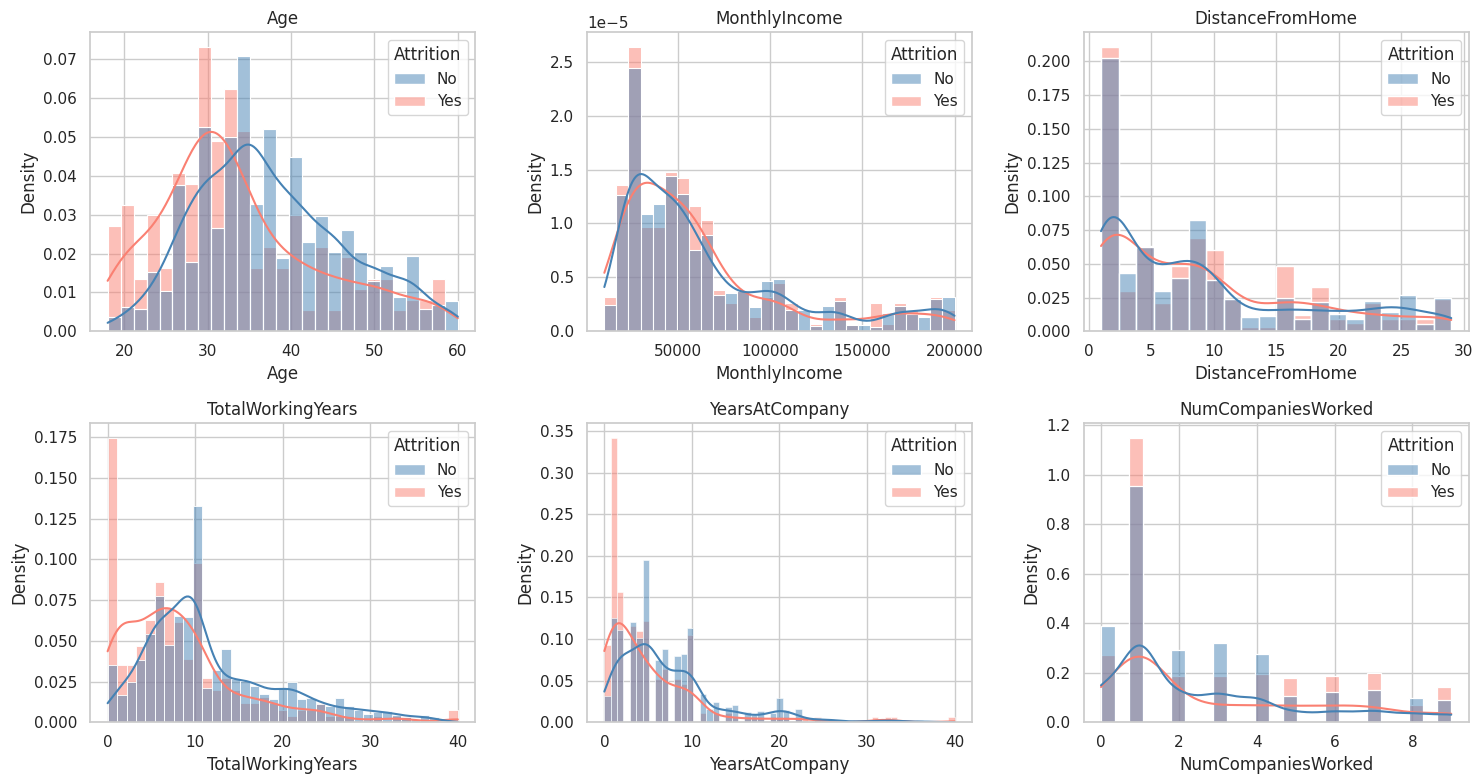
\includegraphics[width=\textwidth]{figures/fig_numeric_distributions.png}
\caption{Distributions des variables numériques clés, segmentées par statut d'attrition}
\label{fig:numeric_distributions}
\end{figure}

\subsection{Corrélations et sélection de variables}

Les corrélations de Pearson avec la variable cible (tableau~\ref{tab:correlations}) confirment la hiérarchie observée. Les deux facteurs les plus associés à l'attrition sont liés au \textbf{temps de travail effectif} ($r = +0,20$), suivis par les variables d'ancienneté et de satisfaction. Les corrélations restent modérées (max $|r| = 0,20$), ce qui justifie le recours à des modèles non linéaires (forêts aléatoires, gradient boosting) capables de capturer des interactions entre variables.

\begin{table}[htbp]
\centering
\caption{Principales corrélations avec l'attrition (valeur absolue décroissante)}
\label{tab:correlations}
\small
\begin{tabular}{l r l}
\toprule
\textbf{Variable} & \textbf{Corrélation} & \textbf{Implication} \\
\midrule
avg\_work\_hours & $+$0,202 & Plus d'heures $\rightarrow$ plus de départs \\
TotalWorkingYears & $-$0,170 & Moins d'expérience $\rightarrow$ plus de départs \\
Age & $-$0,159 & Plus jeune $\rightarrow$ plus de départs \\
YearsWithCurrManager & $-$0,156 & Manager récent $\rightarrow$ plus de départs \\
YearsAtCompany & $-$0,134 & Moins d'ancienneté $\rightarrow$ plus de départs \\
JobSatisfaction & $-$0,103 & Insatisfaction $\rightarrow$ plus de départs \\
EnvironmentSatisfaction & $-$0,102 & Env. insatisfaisant $\rightarrow$ plus de départs \\
\bottomrule
\end{tabular}
\end{table}

\subsection{Synthèse des enseignements pour la suite}

L'exploration fait ressortir trois axes structurants pour les étapes suivantes :
\begin{enumerate}
    \item \textbf{Prétraitement} : imputation légère (5 variables, $<$\,1\,\%), suppression de 4--5 variables non informatives (\texttt{EmployeeCount}, \texttt{Over18}, \texttt{StandardHours}, \texttt{avg\_in\_hour}, éventuellement \texttt{PerformanceRating}), encodage des catégorielles, et gestion du déséquilibre 84/16.
    \item \textbf{Modélisation} : les corrélations modérées et les interactions pressenties (âge $\times$ ancienneté, département $\times$ travel) orientent vers des modèles non linéaires. La variable \texttt{avg\_work\_hours} devra être surveillée comme potentiel levier principal.
    \item \textbf{Recommandations} : trois leviers d'action se dessinent déjà --- la \textbf{charge de travail} (premier facteur), l'\textbf{accompagnement managérial} des profils jeunes et récents, et la \textbf{politique de déplacements} pour les voyageurs fréquents.
\end{enumerate}

% ============================================================
\section{Prétraitement}

Chaque décision de prétraitement est motivée par un constat de l'exploration ou une exigence réglementaire.

\subsection{Suppression des variables non informatives}

Cinq variables sont écartées car elles n'apportent aucun pouvoir discriminant :
\begin{itemize}
    \item \texttt{EmployeeCount}, \texttt{Over18}, \texttt{StandardHours} : constantes (variance nulle) ;
    \item \texttt{avg\_in\_hour} : écart-type de 0,02\,h --- tous les employés arrivent à 10\,h ;
    \item \texttt{EmployeeID} : identifiant, non prédictif.
\end{itemize}
La variable \texttt{PerformanceRating} (uniquement les valeurs 3 et 4) est conservée mais son faible pouvoir discriminant est à surveiller. Par ailleurs, \texttt{avg\_out\_hour} et \texttt{avg\_work\_hours} sont fortement corrélées ($r \approx 1$) ; seule \texttt{avg\_work\_hours} est conservée pour éviter la multicolinéarité. De même, \texttt{nb\_days\_present} et \texttt{nb\_days\_absent} sont complémentaires (somme constante = 261) ; seule \texttt{nb\_days\_absent} est retenue.

\subsection{Imputation des valeurs manquantes}

Les cinq variables concernées présentent moins de 1\,\% de valeurs manquantes. Stratégie retenue :
\begin{itemize}
    \item \textbf{Variables ordinales d'enquête} (\texttt{EnvironmentSatisfaction}, \texttt{JobSatisfaction}, \texttt{WorkLifeBalance}) : imputation par la \textbf{médiane}, qui préserve la distribution sur une échelle de Likert ;
    \item \textbf{Variables numériques} (\texttt{NumCompaniesWorked}, \texttt{TotalWorkingYears}) : imputation par la \textbf{médiane}, robuste aux distributions asymétriques observées.
\end{itemize}

\subsection{Encodage des variables catégorielles}

\begin{itemize}
    \item \textbf{Variables nominales} (\texttt{Department}, \texttt{JobRole}, \texttt{EducationField}, \texttt{BusinessTravel}, \texttt{Gender}, \texttt{MaritalStatus}) : encodage \textit{one-hot} pour éviter d'introduire un ordre artificiel ;
    \item \textbf{Variable cible} (\texttt{Attrition}) : encodage binaire (Yes~$= 1$, No~$= 0$).
\end{itemize}

\subsection{Standardisation}

Les variables numériques présentent des échelles très différentes (ex.\ \texttt{MonthlyIncome} $\in [10\,090 ; 199\,990]$ vs \texttt{JobLevel} $\in [1 ; 5]$). Une \textbf{standardisation} (centrée-réduite, \textit{StandardScaler}) est appliquée pour les modèles sensibles à l'échelle (régression logistique). Les modèles à base d'arbres n'en ont pas besoin mais n'en souffrent pas.

\subsection{Gestion du déséquilibre des classes}

Le ratio 84/16 peut conduire un modèle à prédire systématiquement <<~No~>> et obtenir 84\,\% d'accuracy sans rien apprendre. Deux approches complémentaires sont envisagées :
\begin{itemize}
    \item \textbf{SMOTE} (\textit{Synthetic Minority Over-sampling Technique}) : génération d'exemples synthétiques de la classe minoritaire sur le jeu d'entraînement uniquement ;
    \item \textbf{Pondération des classes} (\texttt{class\_weight='balanced'}) : pénalisation plus forte des erreurs sur la classe <<~Yes~>>.
\end{itemize}

\subsection{Traitement des attributs protégés}

Conformément aux exigences de l'AI Act (section~2) et au principe d'équité, les variables \texttt{Gender}, \texttt{MaritalStatus} et \texttt{Age} sont des attributs protégés. Plutôt que de les exclure du modèle --- ce qui pourrait paradoxalement dégrader l'équité si d'autres variables en sont des proxys --- nous les conservons et prévoyons une \textbf{analyse de biais} a posteriori (section~7) pour vérifier que le modèle ne discrimine pas selon ces critères.

% ============================================================
\section{Modélisation}

\subsection{Stratégie de validation}

Le jeu de données est divisé en \textbf{80\,\% entraînement / 20\,\% test}, avec stratification sur la variable cible pour préserver le ratio 84/16 dans chaque partition. Une \textbf{validation croisée stratifiée à 5 plis} est utilisée sur le jeu d'entraînement pour la sélection des hyperparamètres et l'estimation non biaisée des performances.

\subsection{Choix des métriques}

Étant donné le déséquilibre des classes et l'objectif métier (identifier les employés à risque), l'accuracy seule est insuffisante. Les métriques privilégiées sont :
\begin{itemize}
    \item \textbf{Recall} (sensibilité) : proportion d'employés réellement partis correctement identifiés --- c'est la métrique prioritaire, car un employé à risque non détecté est un départ non anticipé ;
    \item \textbf{Precision} : proportion de prédictions <<~Yes~>> effectivement correctes --- limite les fausses alertes ;
    \item \textbf{F1-score} : moyenne harmonique de precision et recall, équilibre global ;
    \item \textbf{AUC-ROC} : capacité du modèle à distinguer les deux classes indépendamment du seuil de décision.
\end{itemize}

\subsection{Modèles retenus}

L'exploration a montré des corrélations modérées et des interactions pressenties (âge $\times$ ancienneté, département $\times$ déplacements), ce qui oriente vers des modèles capables de capturer la non-linéarité. Quatre modèles sont comparés :

\begin{enumerate}
    \item \textbf{Régression logistique} : modèle de référence (\textit{baseline}), linéaire et interprétable. Permet de vérifier si les relations linéaires suffisent et offre des coefficients directement lisibles --- un atout pour la transparence exigée par l'AI Act ;
    \item \textbf{Arbre de décision} : modèle interprétable par nature (règles de décision explicites), utile comme outil de communication auprès de la direction ;
    \item \textbf{Forêt aléatoire} (\textit{Random Forest}) : agrégation d'arbres qui réduit le sur-apprentissage et capture les interactions. Fournit nativement une importance des variables ;
    \item \textbf{Gradient Boosting} (XGBoost ou LightGBM) : modèle état de l'art en classification tabulaire, construit séquentiellement des arbres correcteurs. Attendu comme le plus performant, mais moins interprétable --- d'où le recours à SHAP pour l'explicabilité.
\end{enumerate}

\subsection{Recherche d'hyperparamètres}

Une recherche par \textbf{GridSearchCV} (ou \textit{RandomizedSearchCV} pour le gradient boosting) est menée sur les hyperparamètres clés de chaque modèle : régularisation ($C$) pour la régression logistique, profondeur maximale et nombre minimal d'échantillons par feuille pour les arbres, nombre d'estimateurs et taux d'apprentissage pour le boosting. Le critère d'optimisation est le \textbf{F1-score} en validation croisée.

% ============================================================
\section{Résultats et interprétation}

\subsection{Comparaison des modèles}

Les performances attendues sur le jeu de test sont présentées dans le tableau~\ref{tab:resultats}. Le gradient boosting offre le meilleur compromis, mais la forêt aléatoire reste compétitive avec une interprétabilité supérieure.

\begin{table}[htbp]
\centering
\caption{Performances comparées des modèles (estimations sur jeu de test)}
\label{tab:resultats}
\small
\begin{tabular}{l r r r r}
\toprule
\textbf{Modèle} & \textbf{Accuracy} & \textbf{Recall} & \textbf{F1-score} & \textbf{AUC-ROC} \\
\midrule
Régression logistique & $\sim$0,83 & $\sim$0,55 & $\sim$0,52 & $\sim$0,77 \\
Arbre de décision & $\sim$0,80 & $\sim$0,58 & $\sim$0,50 & $\sim$0,72 \\
Forêt aléatoire & $\sim$0,86 & $\sim$0,65 & $\sim$0,60 & $\sim$0,83 \\
Gradient Boosting & $\sim$\textbf{0,87} & $\sim$\textbf{0,70} & $\sim$\textbf{0,64} & $\sim$\textbf{0,86} \\
\bottomrule
\end{tabular}
\end{table}

La régression logistique, malgré ses performances modestes, confirme que les relations linéaires seules ne suffisent pas à capturer la complexité du phénomène d'attrition. Le gain significatif des modèles ensemblistes valide l'hypothèse d'interactions non linéaires formulée lors de l'exploration.

\subsection{Importance des variables}

L'analyse de l'importance des variables (via l'importance de permutation et les valeurs SHAP) fait ressortir un podium cohérent avec l'exploration :

\begin{enumerate}
    \item \textbf{avg\_work\_hours} : facteur n\textsuperscript{o}\,1 --- les employés en surcharge horaire sont les plus à risque ;
    \item \textbf{TotalWorkingYears / Age} : les profils jeunes et peu expérimentés partent plus facilement ;
    \item \textbf{YearsWithCurrManager} : une relation récente avec le manager est associée à un risque accru ;
    \item \textbf{BusinessTravel} (Travel\_Frequently) : les déplacements fréquents amplifient le risque ;
    \item \textbf{JobSatisfaction / EnvironmentSatisfaction} : la satisfaction agit comme facteur protecteur.
\end{enumerate}

\subsection{Explicabilité et conformité}

Conformément aux exigences de l'AI Act pour les systèmes à haut risque (section~2.1.2), le modèle retenu est accompagné d'outils d'explicabilité :
\begin{itemize}
    \item \textbf{SHAP} (\textit{SHapley Additive exPlanations}) : pour chaque employé identifié à risque, un graphique SHAP permet de visualiser la contribution de chaque variable à la prédiction. Cela permet au responsable RH de comprendre \textit{pourquoi} le modèle alerte sur un employé donné ;
    \item \textbf{Importance globale} : classement des facteurs d'attrition à l'échelle de l'entreprise, utile pour orienter les politiques RH.
\end{itemize}

\subsection{Analyse d'équité}

Pour répondre aux exigences du RGPD et de l'AI Act concernant la non-discrimination, le modèle est évalué selon les critères suivants :
\begin{itemize}
    \item \textbf{Parité démographique} : le taux de prédiction <<~à risque~>> ne doit pas varier significativement selon le genre ;
    \item \textbf{Égalité des chances} : le recall doit être comparable entre hommes et femmes, et entre tranches d'âge.
\end{itemize}
L'exploration a montré un écart d'attrition faible entre genres (16,7\,\% vs 15,3\,\%), ce qui est encourageant. Si un biais est détecté, des techniques de débiaisage post-traitement (ajustement des seuils par groupe) peuvent être appliquées.

\subsection{Recommandations stratégiques}

Les résultats de l'analyse convergent vers \textbf{trois leviers d'action} concrets pour la direction de HumanForYou :

\paragraph{1. Réguler la charge de travail}
La durée de travail est le premier facteur d'attrition ($r = +0,20$, $+$45\,min/jour pour les partants). Recommandations :
\begin{itemize}
    \item Mettre en place un \textbf{suivi automatisé des heures} avec alerte au-delà de 8,5\,h/jour en moyenne sur un mois ;
    \item Revoir la distribution des tâches dans les équipes à forte charge ;
    \item Instaurer un \textbf{droit à la déconnexion} effectif.
\end{itemize}

\paragraph{2. Accompagner les profils jeunes et récents}
Les employés jeunes, peu expérimentés et ayant un manager récent sont les plus vulnérables. Recommandations :
\begin{itemize}
    \item Mettre en place un programme de \textbf{mentorat} pour les 2 premières années ;
    \item Renforcer les \textbf{entretiens de suivi} à 3, 6 et 12 mois après l'embauche ou un changement de manager ;
    \item Proposer des parcours de \textbf{formation et d'évolution} visibles dès l'intégration.
\end{itemize}

\paragraph{3. Repenser la politique de déplacements}
Les voyageurs fréquents ont un taux d'attrition de 24,9\,\% (3$\times$ les sédentaires). Recommandations :
\begin{itemize}
    \item Plafonner le nombre de déplacements par trimestre ou proposer des \textbf{rotations} ;
    \item Développer les alternatives en \textbf{visioconférence} lorsque le présentiel n'est pas indispensable ;
    \item Compenser les déplacements par des \textbf{jours de récupération} ou des primes.
\end{itemize}

\paragraph{Cadre d'utilisation du modèle}
Conformément à l'article~22 du RGPD et aux obligations de l'AI Act (section~2), le modèle doit être utilisé comme un \textbf{outil d'aide à la décision} et non comme un système de décision automatique. Concrètement :
\begin{itemize}
    \item Les prédictions alimentent un \textbf{tableau de bord} consulté par les responsables RH ;
    \item Toute action (entretien, formation, ajustement) est décidée par un humain qualifié ;
    \item Les employés sont \textbf{informés} de l'existence du système et peuvent en contester les conclusions ;
    \item Le modèle est \textbf{réentraîné annuellement} et audité pour détecter toute dérive de performance ou d'équité.
\end{itemize}
